%%% -*- coding; utf-8 -*-

\documentclass{beamer}

\usepackage{beamerthemesplit}
\usepackage{ucs}
\usepackage[utf8]{inputenc}
\usepackage[francais]{babel}
\usepackage[procnames]{listings}
\usepackage{color}
\usepackage{graphicx}

%\usetheme{classic} %sidebar}
%\usetheme{Singapore}
%\usetheme{shadow}
%\usetheme{Malmoe}
\usetheme{Rochester}


\title{MarkdownMail}
\author{Stéphane Blondon}
\date{\today}
\institute{Yaal}

\begin{document}

\definecolor{keywords}{RGB}{255,0,90}
\definecolor{comments}{RGB}{0,0,113}
\definecolor{red}{RGB}{160,0,0}
\definecolor{green}{RGB}{0,150,0}
 
\lstset{language=Python, 
        basicstyle=\ttfamily\small, 
        keywordstyle=\color{keywords},
        commentstyle=\color{comments},
        stringstyle=\color{red},
        showstringspaces=false,
        identifierstyle=\color{green},
        procnamekeys={def,class}}



\frame{\titlepage}

%\section[Outline]{}
%\frame{\tableofcontents}


\section{Besoin}
\begin{frame}
\frametitle{Besoin}

2 contraintes :
  \begin{itemize}
    \item<1-> créer et maintenir des e-mails facilement
    \item<2-> au rendu agréable pour l'utilisateur
  \end{itemize}

\end{frame}


\section{Besoin}
\begin{frame}
\frametitle{Choix insatisfaisants}

3 choix possibles :
  \begin{itemize}
    \item<1-> mail txt uniquement : facile mais rendu basique
    \item<2-> mail html uniquement : problème pour certains lecteurs de e-mail et antispam. Contraire à la norme
    \item<3-> mail txt et html : difficulté de maintenance
  \end{itemize}

\end{frame}

\begin{frame}[fragile]
\frametitle{Solution}
MarkdownMail utilise un seul contenu, au format Markdown :
    
  \begin{itemize}
    \item<1-> verbatim pour la partie txt,
    \item<2-> converti en html pour la partie html.
  \end{itemize}

\end{frame}

\begin{frame}[fragile]
\frametitle{Installation}
dans un virtualenv :
\begin{verbatim}
pip install markdownmail
\end{verbatim}

disponible en python 2 et 3

sous licence MIT
\end{frame}


\begin{frame}[fragile]
\frametitle{Utilisation}
\begin{lstlisting}
CONTENU = """
PyCon-fr 2016
=============

Infos diverses
--------------

Hop, une liste :

1. lieu : Rennes
2. date : du 13 au 16 octobre
3. merci aux orgas !
"""
\end{lstlisting}

\end{frame}

\begin{frame}[fragile]
\frametitle{Utilisation}
\begin{lstlisting}
email = markdownmail.MarkdownMail(
    from_addr='alice@example.org',
    to_addr='bob@example.org',
    subject='Conf Python',
    content=CONTENU
)

email.send('localhost')
\end{lstlisting}

\end{frame}


\begin{frame}
\frametitle{Résultat}
Le rendu dans Roundcube

\begin{figure}[b]
    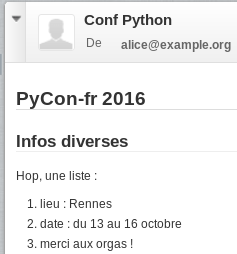
\includegraphics[scale=0.5]{capture_roundcube.png}
\end{figure}
\end{frame}


\begin{frame}
\frametitle{Quelques détails}

  \begin{itemize}
    \item Juste de la colle entre les bibliothèques Markdown et Envelopes
    \item Intégrable facilement dans un service web, script indépendant, etc.
    \item Pas conçu pour des e-mails fortement personnalisés
    \item Pas de pièce jointe actuellement
  \end{itemize}

\end{frame}


\begin{frame}
\frametitle{Page web}
\begin{center}
https://pypi.python.org/pypi/markdownmail
\end{center}

\end{frame}

\end{document}

